\chapter{Implementation Broker}

\section{Protocol implementation}
\label{sec-protocol}
First of all we started to implement the Kafka protocol \todo{ref}
as data basis for all further functionality. The definition of the original
protocol is given as context free grammar for the request and response binary
format. Therefore it seemed likely to adopt the rules of the grammar to our
protocol implementation by map them with the Haskell type system. In a second
step we implemented encoder and decoder functions for getting messages from data
structure to binary format and backwards. 

Therefore our protocol implementation consists of the following modules: 
\begin{itemize}
    \item {Types: Mapping the protocol definition with Haskell type system. }
    \item {Decode: Provide functions to parse binary data to valid structure. }
    \item {Encode: Provide functions to serialize a given structure to a binary
        format. }
\end{itemize}

\subsection{Types}
The design of the Apache Kafka protocol allows to make a distinction between three kind of types:
\begin{enumerate}
  \item Related to request
  \item Related to response
  \item Related to data (for either request or response but can also be used for the \fnurl{Apache Kafka Log}{http://kafka.apache.org/documentation.html\#log} component since log files (on-disk) hold the same structure)
\end{enumerate}

As mentioned before, the representation of the protocol structure is implemented using the Haskell \fnurl{type
system}{https://wiki.haskell.org/Type}, more concrete using data types created
for our need using the named fields - also known as \fnurl{record
syntax}{http://en.wikibooks.org/wiki/Haskell/More_on_datatypes}. Given this, a
further step of abstraction is introduced by creating types for the binary
representation of a protocol field. 

The actual type for the data fields in the protocol have to match an unsigned
integer type of its length. This can easily be done using the
\fnurl{Data.Word}{http://hackage.haskell.org/package/base-4.7.0.2/docs/Data-Word.html}
library. However, while repetitive writing \textit{WordX} (where is stands for
8-, 16-, 32-, or 64 bit) is rather intuitive, creating aliases using the
\textit{type} keyword will result in better readable code, as well as structure
of the implemented protocol. 

%\subsubsection{Batching}
A significant characteristic of the Kafka protocol is the ability to optimize
efficiency due to the batching of multiple message in one single request. Both
the API to send messages and the API to consume messages always work with a
sequence of messages and not only a single message. It is also possible to batch
messages across multiple topics and partitions. It is task of the client
implementation to use this ability clever but it also can ignore it and sends everything
one at a time. Batching leads to sequences of the same type in one request or response. Within
the protocol format this is defined by an array type. In our protocol
implementation the batching sequences are implemented with Haskell lists which
contains N repetitions of another type. Sequences can also be nested. 

As example, the following grammar rule of the original definition shows the
support of batching in the protocol. A batching sequence of a structure A is
shown as [A]:
\begin{lstlisting}
ProduceRequest => 
    RequiredAcks Timeout [TopicName [Partition MessageSetSize MessageSet]]
\end{lstlisting}

Sumarized, all protocol related types are size delimited and
are made up of the following primitive types: 
\begin{table}[H]
    \begin{tabular}{| p{3cm}| p{7cm} | l |}
\hline
\textbf{Type} & \textbf{Description} & \textbf{Implementation Haskell} \\ \hline
Fixed Width Primitives     & Signed integers stored in big endian order.
& Data.Word8, Word16, Word32, Word64 \\ \hline
Variable Length Primitives & Consist of a signed integer giving a length N
followed by N bytes of content. A length of -1 indicates null. String uses an
int16 for its size, and bytes uses an int32.        & Data.ByteString(.Lazy)             \\ \hline
Arrays                     & Repeated structures. Always be encoded as an int32
size containing the length N followed by N,repetitions of the structure which
can itself be made up of other,primitive types & Data.List                          \\ \hline
\end{tabular}
\end{table}

\subsubsection{Types related to request}
Each request and response has its same header fields independent for which api they are used. 
The last part of the format (either request or response) is individual to the particular api which is used. 
\begin{figure}[H]
    \centering
    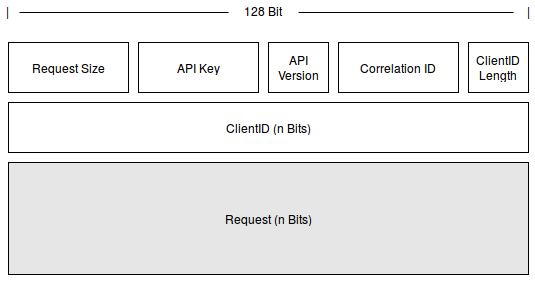
\includegraphics[width=0.7\textwidth]{images/protocol-request-header.png}
    \caption{Common Request Header}
    \label{fig:protocol-request-header.png}
\end{figure}

\subsubsection{Types related to response}
\begin{figure}[H]
    \centering
    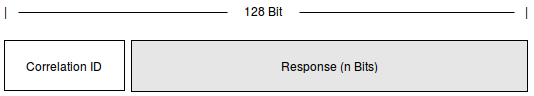
\includegraphics[width=0.7\textwidth]{images/protocol-response-header.png}
    \caption{Common Response Header}
    \label{fig:protocol-response-header.png}
\end{figure}

\subsubsection{Types related to data}
\label{impl-protocol-types-data}
The actual transported data has a common structure,
called a MessageSet. This format happens to be used both for the on-disk storage on the
broker and the on-the-wire format. Therefore the broker do not need to perform
any transformations to the actual message when persisting to the log or read
from it. 

\begin{figure}[H]
    \centering
    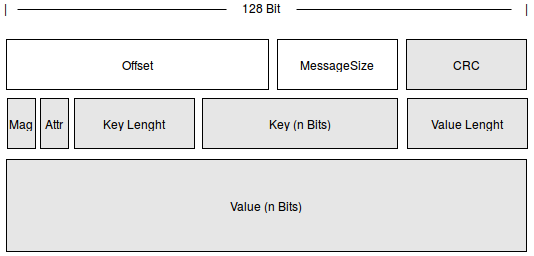
\includegraphics[width=0.7\textwidth]{images/protocol-messageSet.png}
    \caption{MessageSet format as common format for transported data}
    \label{fig:protocol-request-header.png}
\end{figure}

%\subsection{API's}
%\todo{-> verschieben in Kap Kafka detail? }
%\subsubsection{Metadata API}
%Describes the currently available brokers, their host and port information, and
%gives information about which broker hosts which partitions.


%\subsubsection{Fetch API}
%Fetchs / Consumes messages from the broker.
%\subsubsection{Offset API}
%Get information about the available offsets for a given topic partition

%\textbf{Not implemented yet}

%\subsubsection{Offset Commit API}
%Commit a set of offsets for a consumer group

%\textbf{Not implemented yet}

%\subsubsection{Offset Commit API}
%Fetch a set of offsets for a consumer group

%\textbf{Not implemented yet}
\subsubsection{Naming convention}
As for request and response related types we had to introduce an own naming
convention. As a matter of fact, not every field of some kind of request or
response will be unique. For more than once, there is a field that will
represent a \textit{topicName} for example. Thus, naming the field \textit{
topicName} would have been the obvious solution but since the record syntax in
Haskell won't allow to use the same name for a field twice - even in different
data types - we defined unique prefixes for each request and response as being
listed in the following table:

\begin{table}[h]
\centering
\begin{tabular}{|l|l|l|}
\hline
\textbf{API}            & \textbf{Request (Rq)} & \textbf{Response (Rs)} \\ \hline
Metadata API (Md)       & MetadataRequest       & MetadataResponse       \\ \hline
Produce API (Pr)        & ProduceRequest        & ProduceResponse        \\ \hline
Fetch API (Ft)          & FetchRequest          & FetchResponse          \\ \hline
Offset API (Of)         & OffsetRequest         & OffsetResponse         \\ \hline
Offset Commit API (Ofc) & OffsetCommitRequest   & OffsetCommitResponse   \\ \hline
Offset Fetch API (Oft)  & OffsetFetchRequest    & OffsetFetchResponse    \\ \hline
\end{tabular}
\end{table}

%\subsubsection{Example}
As a result, a typical data type is described as follows, while details are
hidden for demonstration purposes.:

\begin{lstlisting}
-- more
data Partition =
    ----------------------
    -- ProduceRequest (pr)
    ----------------------
    RqPrPartition
    { rqPrPartitionNumber :: !PartitionNumber
    , rqPrMessageSetSize  :: !MessageSetSize
    , rqPrMessageSet      :: [MessageSet]
    }
    |
    ----------------------
    -- FetchRequest (ft)
    ----------------------
    RqFtPartition
    { rqFtPartitionNumber :: !PartitionNumber
    , rqFtFetchOffset     :: !Offset
    , rqFtMaxBytes        :: !MaxBytes
    }
    |
-- more
\end{lstlisting}

\subsection{Decode}
There are libraries in Haskell to encode or decode data to or from binary format. 
As for binary serialization, we rely the
\fnurl{Data.Binary}{https://hackage.haskell.org/package/binary-0.4.1/docs/Data-Binary.html}
library. Using the Get Monad (Data.Binary.Get) we are able to comfortably parse
ByteString in it's big endian network order and decode it to appropriate types.
The resulting functions remind of the original definition of the Kafka protocol
as grammar. 

As mentioned in previous section, every request or response has its same header
fields. We provide a general function one for parsing a request and another for
parsing a response. To determine the actual type of request, the protocol describes
an API Key field which holds a numeric code which explicitly defines the type of
request. Depending on the API key further parse functions will be called. The
following code shows the function for parsing a request: 
\begin{lstlisting}
import Data.Binary.Get

requestMessageParser :: Get RequestMessage 
requestMessageParser = do 
    apiKey        <- getWord16be
    apiVersion    <- getWord16be
    correlationId <- getWord32be
    clientIdLen   <- getWord16be
    clientId      <- getByteString $ fromIntegral clientIdLen
    request       <- case (fromIntegral apiKey) of
        0 -> produceRequestParser
        1 -> fetchRequestParser
        3 -> metadataRequestParser
        -- ... further API Codes 
        _ -> -- Invalid API Key 
    return $ RequestMessage apiKey apiVersion correlationId clientIdLen
    clientId request
\end{lstlisting}

Batching sequences are parsed as List whereas we implemented a general function
which gets the list size (number of elements) and a parse function: 
\begin{lstlisting}
parseList :: Int -> (Get a) -> Get [a]
parseList i p = do 
  if (i < 1) 
    then return []
    else do x <- p
            xs <- parseList (i-1) p
            return (x:xs)
\end{lstlisting}

Because the format of a MessageSet is common for the transmission on wire as
well for the persistence in the log we can use the same functions for both use cases:
\begin{lstlisting}
payloadParser :: Get Payload
payloadParser = do
  magic  <- getWord8
  attr   <- getWord8
  keylen <- getWord32be
  paylen <- getWord32be
  payload <- getByteString $ fromIntegral paylen
  return $! Payload magic attr keylen paylen payload

messageParser :: Get Message 
messageParser = do 
  crc    <- getWord32be
  p      <- payloadParser
  return $! Message crc p

messageSetParser :: Get MessageSet 
messageSetParser = do 
  offset <- getWord64be
  len <- getWord32be 
  message <- messageParser
  return $! MessageSet offset len message
\end{lstlisting}

A batched sequence of MessageSets is a special case where the protocol does not provide a
field which determines the number of elements. There is just a field which contains
the size in bytes of all message sets. Therefore we implemented an according
list decoder for sequences of MessageSets:
\begin{lstlisting}
parseMessageSets :: Int -> Get [MessageSet]
parseMessageSets i = do
    if (i < 1)
    then return []
    else do x <- messageSetParser
            xs <- parseMessageSets $ i - (fromIntegral $ length \$ buildMessageSet x)
            return (x:xs)
\end{lstlisting}

\subsection{Encode}%
Obviously the encode module provides the opposite functionalities as the decode
module and was separated just for clarity. Thus we also rely on
\fnurl{Data.Binary}{https://hackage.haskell.org/package/binary-0.4.1/docs/Data-Binary.html}
and use the Put Monad (Data.Binary.Put) to construct ByteStrings.

TODO: Build Request / Response

TODO: Build List 

Analog to the decode functions for MessageSets, the encode functions are
used for request or responses as well for the persistence format for the log:

\begin{lstlisting}
buildldPayload :: Payload -> BL.ByteString 
buildPayload e = runPut $ do 
  putWord8    $ magic e
  putWord8    $ attr e
  putWord32be $ keylen $ e
  putWord32be $ payloadLen  e
  putByteString $ payloadData e

buildMessage :: Message -> BL.ByteString
buildMessage e = runPut $ do 
  putWord32be $ crc e
  putLazyByteString $ buildPayload $ payload e 

buildMessageSet :: MessageSet -> BL.ByteString
buildMessageSet e = runPut $ do 
  putWord64be $ offset e
  putWord32be $ len e
  putLazyByteString $ buildMessage $ message e
\end{lstlisting}

\section{Client Library}

\section{Network Layer}

%One of the most fundamental parts of a message broker are sockets. While a
socket is an endpoint of a bidirectional inter-process communication flow, each
connection established to the broker is basically a socket connection. That
being said, it is important to provide a reliable socket server implementation
which will serve correctly under a heavy load. Haskell provides full control
over sockets using the
\fnurl{Network.Socket}{https://hackage.haskell.org/package/network-2.3.0.7/docs/Network-Socket.html}
module which exposes the \fnurl{C socket
API}{http://pubs.opengroup.org/onlinepubs/7908799/xns/syssocket.h.html}.

\subsection{Socket connection establishment}

The following figure (\ref{fig:broker-activity}) shows the abstract view of how
the socket connection between a client and the broker establishes so that a
communication between those two counterparts can proceed.

\begin{figure}[H]
    \centering
    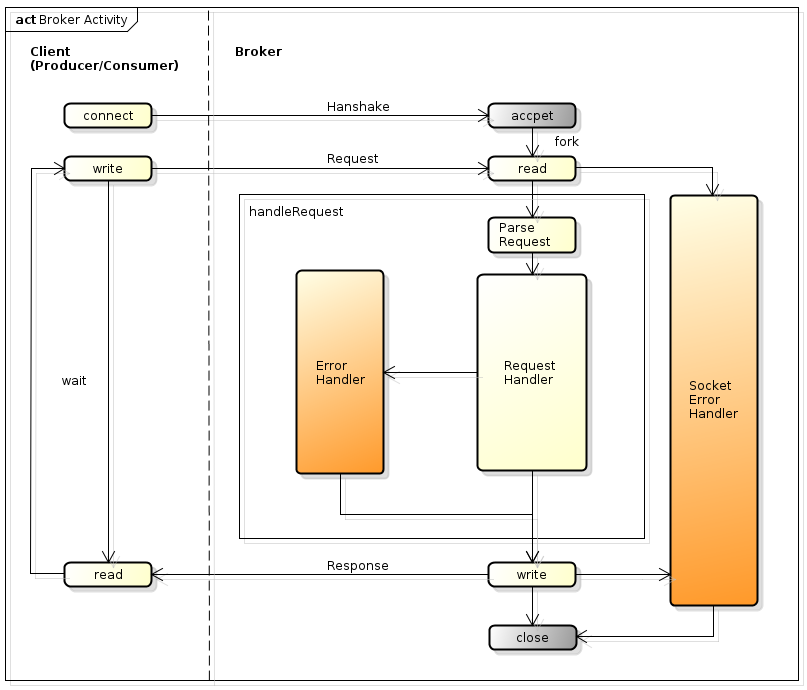
\includegraphics[width=0.7\textwidth]{images/broker-activity.png}
    \caption{Broker request handling concept}
    \label{fig:broker-activity}
\end{figure}

\subsubsection{Create Socket}

First of all, the initialization process of a socket happens on the server by providing the following configuration parameters:
\begin{description}
  \item[Protocol Familiy] \textit{AF\_INET}, for network protocol IPv4
  \item[Socket Type] \textit{Stream}, which provides sequenced, reliable, two-way, connection-based byte streams.
  \item[Protocol Number] \textit{0}, which indicates that the caller does not want to specify the protocol and will leave it up to the service provider.
\end{description}

\subsubsection{Bind Socket}

After the configuration is set, the socket has to be associated with an address
structure which is a constellation of an IP Address and Port. The constructor
\textit{SockAddrInet} of the data type \textit{SockAddr} takes the following
two arguments:

\begin{description}
  \item[Port Number] 4343
  \item[Host Address] iNADDR\_ANY, which binds the socket to all interfaces
\end{description}

TODO: static but could be done with dynamic configuration

\subsubsection{Listen}

While the socket is created and bound to an interface, the socket state can be
entered into listening state. The only configuration parameter which has to be
considered is the maximum number of queued connections they are requesting to
be accepted -- also called backlog. While this parameter is not critical in the
constellation of this broker, we set the queue length to \textbf{50}, which is
also the default value in the Java SocketServer implementation. \textit{Note,
that the focus remains on the amount of data being processed rather than the
number of clients being served.}

\subsection{Receive data}
To receive data from socket buffer we use the function recv from
\fnurl{Network.Socket.ByteString.Lazy}{https://hackage.haskell.org/package/network-2.3.0.1/docs/Network-Socket-ByteString-Lazy.html}
library which provides access to the unix socket interface. Because we work
with a binary protocol and need to parse the data from binary data directly,
this module is much more efficient than the string based network functions. We
take the lazy variant of the library because the input gets directly parsed by
our lazy based encoder \todo{ref}.

Because we want to handle each request individually we explicitly read
only the exact amount of bytes which is needed get one particular request from
the socket buffer. To get the size of a whole request we read the first four
bytes which determines the request size according to the protocol and parse it
to an numeral value.

\begin{lstlisting}
import qualified Network.Socket.ByteString.Lazy as S 
import qualified Data.ByteString.Lazy as BL

recvFromSock :: (Socket, SockAddr) -> IO BL.ByteString
recvFromSock (sock, sockaddr) =  do 
    respLen <- S.recv sock (4 :: Int64
    let parsedLen = getLength respLen
    req <- recvExactly sock parsedLength 
    where
        getLength = runGet $ fromIntegral <$> getWord32be
\end{lstlisting}

After getting the size of a particular request, this determined amount of bytes
is received from socket. Because of the blocking semantics of unix sockets and
tcp packet fragmentation it is not guaranteed, that the len argument to the recv
system call gets the exactly number of bytes of the whole request. The call may produce
less data than specified. Therefore we implement the following function to get
the data in
chunks until the entire request is read. 

\begin{lstlisting}
recvExactly :: Socket -> Int64 -> IO BL.ByteString 
recvExactly sock size = BL.concat . reverse <$> loop [] 0 
  where
    loop chunks bytesRead
        | bytesRead >= size = return chunks
        | otherwise = do  
            chunk <- S.recv sock (size - bytesRead)
            if BL.null chunk 
              then return chunks 
              else loop (chunk:chunks) $! bytesRead + BL.length chunk 
\end{lstlisting}

\subsection{Send data}


\section{API Layer}

\begin{figure}[H]
    \centering
    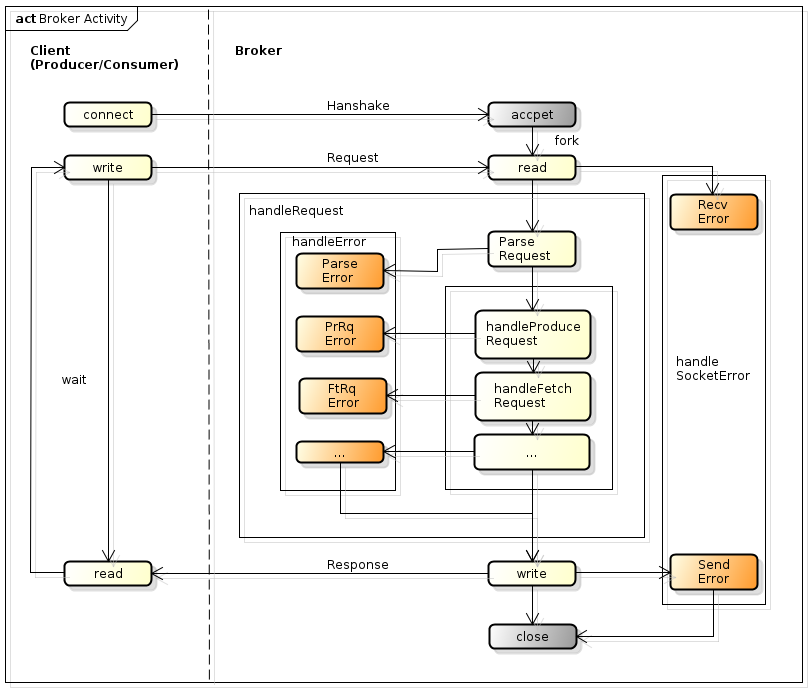
\includegraphics[width=0.7\textwidth]{images/broker-activity-detail.png}
    \caption{Broker request handling concept in detail}
    \label{fig:broker-activity-detail.png}
\end{figure}


\section{Log}

\subsection{Indexing}

\subsection{Storage Layout}
\label{broker-storage}

\subsubsection{Folder structure}

The storage layout is exactly the same as the one defined for for Apache Kafka.
\todo{link} As for now, the root location of the log is not configurable and
set to the folder named \textbf{./log} within the installation directory of the
broker. Each folder represents a partition of a specific topic whereas the name
of the folder is a combination of the topic name and the partition number. 

For example the topic named \textit{myTopic} with the partitions \textit{0} and
\textit{1} will result in the following folder structure:

\begin{itemize}
    \item ./log/myTopic\_0
    \item ./log/myTopic\_1
\end{itemize}

\subsubsection{Files}

There are two types of files they reside within the folder that specifies the
topic and partition (see folder structure):

\begin{description}
    \item[.index] Containing a sequence of index entries
    \item[.log] Containing a sequence of log entries
\end{description}

Both of the file types hold the same name which stays for the base offset and
can be considered as an unique identifier representing a 64 bit integer as a 20
character file name. As it was defined for Apache Kafka, the base offset is the
offset of the first log entry. For example if a log holds messages whereas the
first message has the offset \textit{5 :: Int64} the file name of this log will
be \textit{00000000000000000005.log} and the related index file
\textit{00000000000000000005.index}.

Using this naming convention and by
viewing multiple log files one can extract information about what range of
messages reside in which log. This is a very efficient way to perform a lookup
which is needed for example to append new log messages or archive old messages.

\subsubsection{Index on-disk format}

An index entry consists of the following two fields whereas both of them are 4 bytes each:

\begin{description}
    \item[Relative offset] 4 Bytes offset relative to the base offset (file name)
    \item[Physical position] 4 Bytes physical offset relative to the beginning of the log file
\end{description}

The relative offset of an index entry added with it's base offset represents an
actual message within the log. The second information, the physical position then tells on what 
position the message resides within the log. Thus, log access of O(n) becomes possible.

\subsubsection{Log on-disk format}

The log contains a sequence of log entries whereas the on-disk format of a log
entry is is part of the reason why the Apache Kafka becomes that valuable. In
fact, the on-disk format is exactly the same as the format of the MessageSet
(see \ref{impl-protocol-types-data}) transmitted with a ProduceRequest
\todo{add requests to protocol and link this}. Thus, data does not have to be
modified in any way and can directly be extracted and written to the file
system.

\todo{move the below to protocol}
- log entry: N (4 byte integer -> message length) followed by message (N message bytes)
- message: unique identifier (64 bit integer offset -> byte position of the start of this message in the stream of all messages ever sent to that topic on that partition)

On-disk format of a message:

offset: 8 bytes
message length : 4 bytes (value: 1+4+n) 
magic value  : 1 byte
crc            : 4 bytes
payload        : n bytes
    ?:              : 1 byte
    ?:              : 4 bytes
    message length  : 4 bytes
    message         : n bytes

\subsection{Types}

\begin{table}[H]
\resizebox{\textwidth}{!}{%
\begin{tabular}{|l|l|l|}
\hline
\textbf{Type synonym} & \textbf{Parameter}           & \textbf{Description}                     \\ \hline
TopicStr              & String                       & Parsed topic name as String              \\ \hline
PartitionNr           & Int                          & Parsed partition number as Int           \\ \hline
FilemessageSet        & {[}MessageSet{]}             &                                          \\ \hline
OffsetIndex           & {[}OffsetPosition{]}         &                                          \\ \hline
LogSegment            & (Log, OffsetIndex)           &                                          \\ \hline
RelativeOffset        & Word32                       & 4 Byte offset relative to the BaseOffset \\ \hline
FileOffset            & Word32                       & 4 Byte physical offset of a Log file     \\ \hline
OffsetPosition        & (RelativeOffset, FileOffset) & Tuple of relative and physical offset    \\ \hline
BaseOffset            & Int                          & 8 Byte offset as Int                     \\ \hline
\end{tabular}
}
\end{table}

\subsection{Write a log}

Writing data, type of MessageSet \todo{ref to type}, to a log is the
fundamental process behind the scenes of handling a ProduceRequest \todo{ref
to request}. But before actually writing data to the file system, several
steps come in between and will contribute significantly to the concept of
Apache Kafka's Log system \todo{ref to kafka log}. This section describes
the implementation details of the mentioned steps in the order of occurrence.

\subsubsection{Base Offset}

The incoming request -- which is at this point already parsed -- contains the
topic as well as the partition number for the given set of messages. Thus, we
can identify the location of the related log file. Given the location only, we yet do
not know which file we actually have to.
The file we want to write to is the one named after the highest offset,
which is why we do not get around reading the content of this directory. While doing so,
string transformations have to be applied to identify the correct offset and thus the
file to write to. Handling the case where no file exists leads
to the creation of a new log with the offset of zero.
\\

Before applying filters and string transformations, the list of files has to be
build. The library
\fnurl{System.Directory}{http://hackage.haskell.org/package/directory-1.2.2.1/docs/System-Directory.html}
provides the function \textit{getDirectoryContents} that takes a file path as a
string and returns a list of all entires in the directory. This operation
performs I/O and thus the return type is an IO monadic value. \textit{As
described on
\fnurl{hackage}{http://hackage.haskell.org/package/directory-1.2.2.1/docs/System-Directory.html\#v:getDirectoryContents},
there are several causes why this operation may fail but at this point, we do
not provide proper error handling.}

Now Haskell can perform it's beauty. To get the list of all offsets within
the directory, the function \textit{offsetFromFileName} extracts the offset
as an \textit{Int} from a \textit{String}. As an example,
\textit{"00000000000000000005.log" :: String } will be transformed to
\textit{0000000000000000005 :: Int}:

\begin{lstlisting}
offsetFromFileName :: [Char] -> Int
offsetFromFileName = read . reverse . snd . splitAt 4 . reverse
\end{lstlisting}

The function \textit{offsetFromFileName} can be mapped over a filtered list of
strings, which will give the list of all offsets within the directory. The
filter function basically omits the files other than the ones ending with
\textit{".log"} as well as the root directories, typically \textit{".", ".."}.


\begin{lstlisting}
getBaseOffsets :: (TopicStr, Int) -> IO [BaseOffset]
getBaseOffsets (t, p) = do
dirs <- getDirectoryContents $ getLogFolder (t, p)
return $ map (offsetFromFileName) (filter (isLogFile) (filterRootDir dirs))
\end{lstlisting}

Finally, the highest offset can be returned. If the list is empty -- and thus no log file 
yet exists within the log folder -- zero will be returned.

\begin{lstlisting}
maxOffset :: [Int] -> Int
maxOffset [] = 0
maxOffset [x] = x
maxOffset xs = maximum xs

getLastBaseOffset :: (TopicStr, Int) -> IO BaseOffset
getLastBaseOffset (t, p) = do
bos <- getBaseOffsets (t, p)
return (maxOffset bos)
\end{lstlisting}

\subsubsection{Last Offset Position}

Given the highest offset for a specific topic name and partition, the next step
leads to determine the latest entry of the index file -- which is named after
this offset. The index file now will be parsed with the regard to identify the
latest offset and physical position of the message that lies within the actual
log file. In order to increase I/O performance the index file will be mapped
into memory first using
\fnurl{mmap}{http://man7.org/linux/man-pages/man2/mmap.2.html}. The resulting
memory-mapped file implements demand paging which is an operation that copies a
disk page into physical memory only if an attempt is made to access it or the
page is not already in memory. This comes very handy in terms of Haskell's
laziness such as that a lazy ByteString can be taken as a result of this
operation and thus memory consumption can be considered as moderate. But even
more importantly, the amount of I/O operations will be decreased drastically
for multiple lookups on the index file.

Haskell provides the System.IO.MMap library which is an interface to mmap(2)
system call under POSIX. 

%todo ...DESCRIBE MMAP LIBRARY...

\begin{lstlisting}
getLastOffsetPosition :: (TopicStr, Int) -> BaseOffset -> IO OffsetPosition
getLastOffsetPosition (t, p) bo = do 
  let path = getPath (getLogFolder (t, p)) (indexFile bo)
  -- check if file exists
  bs <- mmapFileByteStringLazy path Nothing
  case decodeIndex bs of
    Left (bs, bo, e)   -> do
        print e
        return (0,0)
    Right (bs, bo, ops) -> return (lastIndex ops)
\end{lstlisting}

%todo describe decodeIndex

\subsubsection{Last Log Offset}

The last offset provided by the index file does not ensure that this is the
last offset above all existing messages within the log. As described in the
storage section (\ref{broker-storage}), index entries are created only after a
certain amount of bytes has been passed. The gap between the last offset of the
index and the last offset of the log will be resolved by parsing the messages
between the two offsets where the last of those messages can finally be
considered as the message that contains the highest offset above all messages. 

Fortunately, the mmap wrapper function \textit{mmapFileByteStringLazy} takes a
\textit{Maybe (Int64, Int64)} to specify the range of the file to be mapped.
The range is defined by the offset, which is the beginning byte of the file
region and the size tells the mapping length.

\begin{lstlisting}
getLastLogOffset :: (TopicStr, Int) -> BaseOffset -> OffsetPosition -> IO Offset
getLastLogOffset (t, p) bo (rel, phys) = do
  let path = getPath (logFolder t p) (logFile bo)
  fs <- getFileSize path
  bs <- mmapFileByteStringLazy path $ Just (fromIntegral phys, (fromIntegral (fs) - fromIntegral phys))
  return (lastOffset $ runGet getLog bs)
\end{lstlisting}

\subsubsection{Append Index}

\subsubsection{Append Log}


\subsection{Read from log}

\subsection{Optimization}

Next to optimizations like batching in the network layer \todo{ref to network},
we do also provide some optimizations in terms of I/O. \todo{Kafka: a
Distributed Messaging System for Log Processing}.

\subsubsection{Page Cache:}

First of all, We therefore avoid to explicitly cache messages in memory but
instead rely on the underlying file system cache. This has the benefit of
avoiding double buffering since messages are only cached in the page cache.
Thus, even if the broker process has to be restarted, the cache retains warm.

\todo{more details on modern os and page cache}

\subsubsection{Sequential I/O: }

While producers and consumers lead the broker to access
segments of files, the actual access which taking place is going to be a
sequential access rather than random. This will reduce seeking time to 1 per
partition. In fact, the broker holds a point on a given offset whereas all
messages below the pointer can be considered as already consumed and all
messages with offset greater than the provided one as unconsumed. Now since
messages are ordered this will lead to a sequential I/O with a constant seeking
time (O(1)).


\subsubsection{Internal data transfer:}

As mentioned earlier, HMB omit explicit caching but instead relies on the file system.
Keep this in mind, the actual network access for consumers can be optimized as well.
While a typical approach to sending bytes from a local file to a remote
socket involves the following steps: 
\begin{enumerate}
  \item Read data from storage (disk)
  \item Copy data from the page cache to an application buffer
  \item Copy application buffer to a kernel buffer
  \item Send kernel buffer to the socket
\end{enumerate}

With the help of the sendfile API \todo{ref} it is possible to transfer bytes
from a file channel to a socket channel, whereas the delivery process will
result in the following steps:

\begin{enumerate}
  \item Read data from storage (disk)
  \item Send data from page cache to the socket
\end{enumerate}


\section{Bootstrapping}
TODO: Main function 

